\documentclass[11pt]{article}

\usepackage{abstract}
\usepackage{algorithm}
\usepackage{algorithmic}
\usepackage{amsmath}
\usepackage{amssymb}
\usepackage{bm}
\usepackage{caption}
\usepackage{CJKutf8}
\usepackage{color}
\usepackage{enumitem}
\usepackage{epsfig}
\usepackage{fancyhdr}
\usepackage{float}
\usepackage{graphics}
\usepackage{graphicx}
\usepackage{geometry}
\usepackage{indentfirst}
\usepackage{lastpage}
\usepackage{listings}
\usepackage{mathdots}
\usepackage{mathpazo}
\usepackage{multirow}
\usepackage{pstricks-add}
\usepackage{pst-blur}
\usepackage{subcaption}
\usepackage{tikz}
\usepackage{wasysym}
\usepackage{xcolor}
\usepackage[BoldFont,SlantFont,CJKsetspaces,CJKchecksingle]{xeCJK}

\allowdisplaybreaks
\DeclareMathOperator*{\argmin}{argmin}
\definecolor{Blue}{rgb}{1.,0.75,0.8}
\definecolor{mygray}{rgb}{0.5,0.5,0.5}
\definecolor{mygreen}{rgb}{0,0.6,0}
\definecolor{mymauve}{rgb}{0.58,0,0.82}
\pagestyle{empty}
\parindent 2em   %段首缩进
\setlength{\parindent}{2em}
\setCJKmainfont[BoldFont=SimHei]{SimSun}
\setCJKmonofont{SimSun}% 设置缺省中文字体
\usetikzlibrary{arrows, automata, calc, shapes}

\newcommand{\HRule}{\rule{\linewidth}{0.5mm}}
\newcommand{\hytt}[1]{\texttt{\hyphenchar\font=\defaulthyphenchar #1}}
\renewcommand{\algorithmicrequire}{\textbf{Input:}}   
\renewcommand{\algorithmicensure}{\textbf{Output:}}  
% \hyphenation{read-Sym-bol re-ad-Space-Tab-New-line str-Tab}

%\footnotesize
\lstset{ %
  backgroundcolor=\color{white},   % choose the background color; you must add \usepackage{color} or \usepackage{xcolor}
  basicstyle=\ttfamily,            % the size of the fonts that are used for the code
  breakatwhitespace=false,         % sets if automatic breaks should only happen at whitespace
  breaklines=true,                 % sets automatic line breaking
  captionpos=b,                    % sets the caption-position to bottom
  commentstyle=\ttfamily\color{mygreen},    
                                   % comment style
  deletekeywords={},               % if you want to delete keywords from the given language
  escapeinside={},                 % if you want to add LaTeX within your code
  extendedchars=true,              % lets you use non-ASCII characters; for 8-bits encodings only, does not work with UTF-8
  frame=single,                    % adds a frame around the code
  keepspaces=true,                 % keeps spaces in text, useful for keeping indentation of code (possibly needs columns=flexible)
  keywordstyle=\color{blue},       % keyword style
  language=C++,                    % the language of the code
  morekeywords={},                 % if you want to add more keywords to the set
  numbers=left,                    % where to put the line-numbers; possible values are (none, left, right)
  numbersep=5pt,                   % how far the line-numbers are from the code
  numberstyle=\tiny\color{mygray}, % the style that is used for the line-numbers
  rulecolor=\color{black},         % if not set, the frame-color may be changed on line-breaks within not-black text (e.g. comments (green here))
  showspaces=false,                % show spaces everywhere adding particular underscores; it overrides 'showstringspaces'
  showstringspaces=false,          % underline spaces within strings only
  showtabs=false,                  % show tabs within strings adding particular underscores
  stepnumber=1,                    % the step between two line-numbers. If it's 1, each line will be numbered
  stringstyle=\color{mymauve},     % string literal style
  tabsize=2,                       % sets default tabsize to 2 spaces
  title=\lstname                   % show the filename of files included with \lstinputlisting; also try caption instead of title
}

\pagestyle{fancy}
\rhead{page \thepage\ of \pageref{LastPage}}
%\chead{}
\lhead{操作系统实验报告}
\cfoot{}

\begin{document}

\title{操作系统实验2 \quad 进程状态}
\author{计算机1202 \quad 张艺瀚\\学号:20123852}
\maketitle

\thispagestyle{fancy}
%\newpage
\normalsize

\section{题目}
模拟进程状态转换及其PCB的变化 

\section{目的}
自行编制模拟程序,通过形象化的状态显示,使学生理解进程的概念、进程之间的状态转换及其所带来的PCB内容、组织的变化,理解进程与其PCB间的一一对应关系。

\section{要求}
\begin{enumerate}
\item 设计并实现一个模拟进程状态转换及其相应PCB内容、组织结构变化的程序。
\item 独立编写、调试程序。进程的数目、进程的状态模型(三状态、五状态、七状态或其它)以及PCB的组织形式可自行选择。
\item 合理设计与进程PCB相对应的数据结构。PCB的内容要涵盖进程的基本信息、控制信息、资源需求及现场信息。
\item 设计出可视性较好的界面,应能反映出进程状态的变化引起的对应PCB内容、组织结构的变化。
\item 代码书写要规范,要适当地加入注释。
\item 鼓励在实验中加入新的观点或想法,并加以实现。
\item 认真进行预习,完成预习报告。
\item 实验完成后,要认真总结,完成实验报告。
\end{enumerate}

\section{程序流程图}
见图\ref{fig: create_destroy}-\ref{fig: activate}

% 流程图定义基本形状
\tikzstyle{startstop} = [rectangle, rounded corners, minimum width=3cm, minimum height=1cm,text centered, draw=black, fill=red!30]
\tikzstyle{io} = [trapezium, trapezium left angle=70, trapezium right angle=110, minimum width=3cm, minimum height=1cm, text centered, draw=black, fill=blue!30]
\tikzstyle{operation} = [rectangle, minimum width=3cm, minimum height=1cm, text centered, draw=black, fill=orange!30]
\tikzstyle{judge} = [diamond, minimum width=3cm, minimum height=1cm, text centered, draw=black, fill=green!30]
\tikzstyle{arrow} = [thick,->,>=stealth]

\begin{figure}[htbp]
\centering
\begin{subfigure}[b]{0.5\textwidth}
\centering
\begin{tikzpicture}[node distance=2cm]
%定义流程图具体形状
\node (a) [operation] at(0,0)       {创建pcb};
\node (b) [operation] at(0,-2)      {设置标识符};
\node (c) [operation] at(0,-4)      {为进程映像分配空间};
\node (d) [operation] at(0,-6)      {初始化pcb};
\node (e) [operation] at(0,-8)      {设置指针(就绪队列和家族树)};

%连接具体形状
\draw [arrow](a) -- (b);
\draw [arrow](b) -- (c);
\draw [arrow](c) -- (d);
\draw [arrow](d) -- (e);
%\draw [arrow]( ) -- node[anchor=east] {是} ( );
%\draw [arrow]( ) -- node[anchor=south] {否} ( );
\end{tikzpicture}
\caption{创建原语}
\label{fig: create}
\end{subfigure}%
~ %add desired spacing between images, e. g. ~, \quad, \qquad, \hfill etc.
%(or a blank line to force the subfigure onto a new line)
\begin{subfigure}[b]{0.5\textwidth}
\centering
\begin{tikzpicture}[node distance=2cm]
%定义流程图具体形状
\node (a) [operation] at(0,0)       {释放内外存};
\node (b) [operation] at(0,-2)      {关闭打开文件};
\node (c) [operation] at(0,-4)      {释放共享内存段和lock};
\node (d) [operation] at(0,-6)      {撤销子孙进程};
\node (e) [operation] at(0,-8)      {释放pcb};

%连接具体形状
\draw [arrow](a) -- (b);
\draw [arrow](b) -- (c);
\draw [arrow](c) -- (d);
\draw [arrow](d) -- (e);
%\draw [arrow]( ) -- node[anchor=east] {是} ( );
%\draw [arrow]( ) -- node[anchor=south] {否} ( );
\end{tikzpicture}
\caption{撤销原语}
\label{fig: destroy}
\end{subfigure}
\caption{创建原语和撤销原语}
\label{fig: create_destroy}
\end{figure}

\begin{figure}[htbp]
\centering
\begin{subfigure}[b]{0.5\textwidth}
\centering
\begin{tikzpicture}[node distance=2cm]
%定义流程图具体形状
\node (a) [operation] at(0,0)       {保护现场};
\node (b) [operation] at(0,-2)      {置进程状态为等待};
\node (c) [operation] at(0,-4)      {将进程插入对应事件的等待队列};
\node (d) [operation] at(0,-6)      {进程调度};

%连接具体形状
\draw [arrow](a) -- (b);
\draw [arrow](b) -- (c);
\draw [arrow](c) -- (d);
%\draw [arrow]( ) -- node[anchor=east] {是} ( );
%\draw [arrow]( ) -- node[anchor=south] {否} ( );
\end{tikzpicture}
\caption{阻塞原语}
\label{fig: block}
\end{subfigure}%
~ %add desired spacing between images, e. g. ~, \quad, \qquad, \hfill etc.
%(or a blank line to force the subfigure onto a new line)
\begin{subfigure}[b]{0.5\textwidth}
\centering
\begin{tikzpicture}[node distance=2cm]
%定义流程图具体形状
\node (a) [operation] at(0,0)       {从对应等待队列中取出进程};
\node (b) [operation] at(0,-2)      {置进程状态为就绪};
\node (c) [operation] at(0,-4)      {将进程插入就绪队列};
\node (d) [operation] at(0,-6)      {进程调度};

%连接具体形状
\draw [arrow](a) -- (b);
\draw [arrow](b) -- (c);
\draw [arrow](c) -- (d);
%\draw [arrow]( ) -- node[anchor=east] {是} ( );
%\draw [arrow]( ) -- node[anchor=south] {否} ( );
\end{tikzpicture}
\caption{唤醒原语}
\label{fig: wakeup}
\end{subfigure}
\caption{阻塞原语和唤醒原语}
\label{fig: block_wakeup}
\end{figure}

\begin{figure}[htbp]
\centering
\begin{tikzpicture}[node distance=2cm]
%定义流程图具体形状
\node (a) [operation] at(-5,0)      {获取进程标识符};
\node (b) [operation] at(-5,-2.5)   {s=进程状态};
\node (c) [judge]     at(-5,-5)     {s=运行?};
\node (d) [operation] at(-5,-7.5)   {停止进程};
\node (e) [operation] at(-5,-10)    {将pcb副本保存到指定内存};
\node (f) [judge]     at(0,-10)     {s=阻塞?};
\node (g) [operation] at(0,-7.5)    {置进程状态为阻塞挂起};
\node (h) [operation] at(5,-7.5)    {置进程状态为就绪挂起};
\node (i) [judge]     at(0,-5)      {s=运行?};
\node (j) [operation] at(0,-2.5)    {进程调度};
\node (k) [operation] at(0,0)       {返回};

%连接具体形状
\draw [arrow](a) -- (b);
\draw [arrow](b) -- (c);
\draw [arrow](c) -- node[anchor=east] {是} (d);
\draw [arrow](c.east) -| node[anchor=south] {否} (-2.5, -8.5) -|  (e.north);
\draw [arrow](d) -- (e);
\draw [arrow](e.south) |- (-3, -12) -| (f.south);
\draw [arrow](f) -- node[anchor=east] {是} (g);
\draw [arrow](f.east) -| node[anchor=south] {否} (3, -10) -| (h.south);
\draw [arrow](g) -- (i);
\draw [arrow](h.north) -- (5, -6.5) -| (i.south);
\draw [arrow](i) -- node[anchor=east] {是} (j);
\draw [arrow](i.east) -| node[anchor=west] {否} (2, -1.5) -| (k.south);
\draw [arrow](j) -- (k);
%\draw [arrow]( ) -- node[anchor=east] {是} ( );
%\draw [arrow]( ) -- node[anchor=south] {否} ( );
\end{tikzpicture}
\caption{挂起原语}
\label{fig: suspend}
\end{figure}

\begin{figure}[htbp]
\centering
\begin{tikzpicture}[node distance=2cm]
%定义流程图具体形状
\node (a) [operation] at(-5,0)      {获取进程标识符};
\node (b) [judge]     at(-5,-2.5)   {就绪挂起?};
\node (c) [operation] at(-5,-5)     {置进程状态为就绪};
\node (d) [operation] at(0,-5)      {置进程状态为阻塞};
\node (e) [judge]     at(-5,-7.5)   {就绪?};
\node (f) [operation] at(-5,-10)    {进程调度};
\node (g) [operation] at(-5,-12.5)  {返回};

%连接具体形状
\draw [arrow](a) -- (b);
\draw [arrow](b) -- node[anchor=east] {是} (c);
\draw [arrow](b.east) -| node[anchor=south] {否} (0, -3) -| (d.north);
\draw [arrow](c) -- node[anchor=east] {是} (e);
\draw [arrow](d.south) -| (0, -6) -| (e);
\draw [arrow](e) -- node[anchor=east] {是} (f);
\draw [arrow](e.east) -| node[anchor=south] {否} (-3, -11) -| (g.north);
\draw [arrow](f) -- (g);
%\draw [arrow]( ) -- node[anchor=east] {是} ( );
%\draw [arrow]( ) -- node[anchor=south] {否} ( );
\end{tikzpicture}
\caption{激活原语}
\label{fig: activate}
\end{figure}

\section{使用的数据结构及其说明}
见表\ref{tab: data_structure}
\begin{table}[htbp]
\centering  % 表居中
\begin{tabular}{lll}  % {lccc} 表示各列元素对齐方式,left-l,right-r,center-c
\hline
名称 & 数据结构 & 说明 \\
\hline  % \hline 在此行下面画一横线
pcb表 & Pcb型(类)数组 & / \\
Pcb & 类 & 属性:进程id,进程名,用户id,cpu状态, \\
        & & 进程状态,优先级,内存,资源 \\
cpu状态 & 枚举类型 & / \\
进程状态 & 枚举类型 & / \\
内存 & 结构类型 & 域:起始地址,内存大小,占用标识位 \\
资源 & 结构 & 域:打开文件数组 \\
等待队列 & 数组 & / \\
阻塞队列 & 数组 & / \\
进程树 & 树 & 类属性:根节点指针 \\
进程树节点 & 类 & 属性:进程id,双亲指针,子女指针数组 \\
\hline
\end{tabular}
\caption{数据结构说明\label{tab: data_structure}}
\end{table}

\section{程序源代码、文档注释及文字说明}
\texttt{thread.cpp}中实现了6种原语,\texttt{pcb.h}中定义了pcb数据结构,\texttt{group\_tree.h}中实现了进程树。具体见代码清单\ref{lst: thread_cpp}-\ref{lst: group_tree_h}:

\begin{center}
\begin{lstlisting}[caption = {\texttt{thread.cpp}代码清单}, label = {lst: thread_cpp}][htbp]
#include <algorithm>
#include <cassert>
#include <cmath>
#include <initializer_list>
#include <iostream>
#include <fstream>
#include <functional>
#include <set>
#include <sstream>
#include <vector>
 
#include "pcb.h"
#include "group_tree.h" 

using namespace std;

const int concurrency = 256;

vector<Pcb> pcb_table;
vector<int> ready_queue;
vector<int> blocked_queue;
int id = 0;
int exe_p;
bool schedule = false;
GroupTree group_tree;

bool get_pcb(string name, int& i){
  // return false: exists; true: not exists
  // i: index (-1, allocate memory failed)
  auto p = find_if(pcb_table.begin(), pcb_table.end(), 
    [name](const Pcb& pcb){
      return pcb.name == name;
    });
  if(p == pcb_table.end()){
    if(pcb_table.size() + 1 > concurrency){
      i = -1;
      cerr << "Outstrip capacity of concurrency, apply for pcb failed!\n";
      return false;
    }else{
      pcb_table.push_back(Pcb());
      i = pcb_table.size() - 1;
      cerr << "Process named \"" << name << "\" not found, create successfully!\n";
      return false;
    }
  }else{
    i = p - pcb_table.begin();
    cerr << "Procdss named\"" << name << "\" already exists.\n";
    return true;
  }
}

bool create(string name, CpuState cpu_state, int priority, MainStore main_store, Resources resources){
  int i;
  if(!get_pcb(name, i) && i != -1){
    pcb_table[i].id = ++id;
    pcb_table[i].priority = priority;
    pcb_table[i].cpu_state = cpu_state;
    pcb_table[i].main_store = main_store;
    pcb_table[i].resources = resources;
    ready_queue.push_back(i);
    // group_tree
    cerr << "Apply pcb successfully.\n";
    return true;
  }else{
    cerr << "Error: create process named \"" << name << "\" failed!\n";
    return false;
  }
}

bool remove(int i){
  if(pcb_table[i].status == ready){
    ready_queue.erase(find_if(ready_queue.begin(), ready_queue.end(),
      [i](const int& idx){
        return i == idx;
      }));
    cerr << "Remove pcb[" << i << "] from ready_queue successfully.\n";
    return true;
  }else if(pcb_table[i].status == blocked){
    blocked_queue.erase(find_if(blocked_queue.begin(), blocked_queue.end(),
      [i](const int& idx){
        return i == idx;
      }));
    cerr << "Remove pcb[" << i << "] from blocked_queue successfully.\n";
    return true;
  }else{
    return false;
  }
}

bool kill(int i){
  if(i >= 0){
    if(pcb_table[i].status == running){
      // stop(i)
      schedule = true;
    }
    remove(i);
    // kill subtree in group_tree
    // release main_store and resources
    pcb_table.erase(pcb_table.begin() + i);
    cerr << "Kill pcb[" << i << "] successfully.\n";
    return true;
  }else{
    cerr << "Error: kill pcb[" << i << "] failed!\n";
    return false;
  }
}

bool destroy(string name){
  schedule = false;
  int i;
  if(get_pcb(name, i)){
    kill(i);
    if(schedule){
      // scheduler dispatches
    }
    cerr << "Destroy process named \"" << name << "\" successfully.\n";
    return true;
  }else{
    cerr << "Error: destroy process named \"" << name << "\" failed!\n";
    return false;
  }
}

bool block(){
  int i = exe_p;
  if(exe_p >= 0)
  {
    // stop(i)
    pcb_table[i].status = blocked;
    blocked_queue.push_back(i);
    // scheduler dispatches
    cerr << "Block successfully.\n";
    return true;
  }else{
    cerr << "Error: block failed!\n";
    return false;
  }
}

bool wake_up(string name){
  int i;
  if(get_pcb(name, i)){
    remove(i);
    pcb_table[i].status = ready;
    ready_queue.push_back(i);
    // scheduler dispatches
    cerr << "Wake up process named \"" << name << "\" successfully.\n";
    return true;
  }else{
    cerr << "Error: wake up process named \"" << name << "\" failed!\n";
    return false;
  }
}

bool suspend(string name){
  int i;
  if(get_pcb(name, i)){
    Status s = pcb_table[i].status;
    if(s == running){
      // stop(i)
    }
    // main_store <- pcb_table[i]
    if(s == blocked){
      pcb_table[i].status == blocked_suspend;
    }else{// ready / running
      pcb_table[i].status = ready_suspend;
    }
    if(s == running){
      // scheduler dispatches
    }
    cerr << "Suspend process named \"" << name << "\" successfully.\n";
    return true;
  }else{
    cerr << "Error: suspend process named \"" << name << "\" failed!\n";
    return false;
  }
}

bool activate(string name){
  int i;
  if(get_pcb(name, i)){
    pcb_table[i].status = pcb_table[i].status == ready_suspend? ready: blocked;
    if(pcb_table[i].status == ready){
      // scheduler dispatches
    }
    cerr << "Activate process named \"" << name << "\" successfully.\n";
    return true;
  }else{
    cerr << "Error: activate process named \"" << name << "\" failed!\n";
    return false;
  }
}

int main(int argc, char** argv){
  group_tree.create(-1, 0);
  group_tree.create(-1, 1);
  group_tree.create(-1, 2);
  group_tree.create(0, 4);
  group_tree.create(4, 5);
  group_tree.create(4, 6);
  group_tree.create(6, 7);
  group_tree.create(1, 3);
  group_tree.preorder_travers_display();
  group_tree.destroy(4);
  group_tree.preorder_travers_display();
  return 0;
}
\end{lstlisting}
\end{center}

\begin{center}
\begin{lstlisting}[caption = {\texttt{pcb.h}代码清单}, label = {lst: pcb_h}][htbp]
#ifndef PCB_H
#define PCB_H

#include <algorithm>
#include <cassert>
#include <cmath>
#include <initializer_list>
#include <iostream>
#include <iterator>
#include <fstream>
#include <functional>
#include <regex>
#include <set>
#include <sstream>
#include <vector>

using namespace std;

enum CpuState{usr_state, kernel_state};
enum Status{creat, ready, ready_suspend, blocked, blocked_suspend, running, ex};
struct MainStore{
  int start_addr;
  int mem_size;
  bool usable;
};
struct Resources{
  vector<string> opened_files;
};

class Pcb{
public:
  Pcb(){}

// description
  int id;
  string name;
  string usr_id;
  // group_tree

// ctrl_infl
  CpuState cpu_state;
  Status status;
  int priority;
  // int entry_addr;
  // int disk_addr;
  // StatInfo stat_info;

// resources
  // main_store
  MainStore main_store;
  Resources resources;

// cpu_scene

private:
};

#endif // PCB_H
\end{lstlisting}
\end{center}

\begin{center}
\begin{lstlisting}[caption = {\texttt{group\_tree.h}代码清单}, label = {lst: group_tree_h}][htbp]
#ifndef GROUP_TREE_H
#define GROUP_TREE_H

#include <algorithm>
#include <cassert>
#include <cmath>
#include <initializer_list>
#include <iostream>
#include <iterator>
#include <fstream>
#include <functional>
#include <regex>
#include <set>
#include <sstream>
#include <vector>

#include "pcb.h"

using namespace std;

struct Node{
  Node(){}
  Node(int n, Node* pp, vector<Node*> cpl):
  pcb_id(n), parent_ptr(pp), child_ptr_list(cpl){}

  int pcb_id;
  Node* parent_ptr;
  vector<Node*> child_ptr_list;
};

class GroupTree{
public:
  GroupTree(){
    root = new Node();
    root->pcb_id = -1;
  }

  void destruct(Node* p){
    if(p != nullptr){
      for(size_t i = 0; i < p->child_ptr_list.size(); ++i){
        destruct(p->child_ptr_list[i]);
      }
      delete p;
    }
  }

  ~GroupTree(){
    destruct(root);
    // cout << "destruct\n";
  }

  void find(int i, Node* p, bool& found, Node*& pp){
    if(p != nullptr){
      if(p->pcb_id == i){
        found = true;
        pp = p;
        return;
      }else{
        for(size_t j = 0; j < p->child_ptr_list.size(); ++j){
          find(i, p->child_ptr_list[j], found, pp);
        }
      }
    }
  }

  bool create(int i, int pcb_id){
    Node* pp;
    bool found = false;
    find(i, root, found, pp);
    // if(pp != nullptr){
    //  cout << "find " << i << " " << pp->pcb_id << endl;
    // }else{
    //  cout << "find null\n";
    // }
    if(found){
      Node* np = new Node();
      np->pcb_id = pcb_id;
      np->parent_ptr = pp;
      pp->child_ptr_list.push_back(np);
    }
  }

  bool destroy(int i){
    Node* p;
    bool found = false;
    find(i, root, found, p);
    if(found){
      p->parent_ptr->child_ptr_list.erase(
        find_if(
          p->parent_ptr->child_ptr_list.begin(), p->parent_ptr->child_ptr_list.end(),
          [i](Node* cp){
            return cp->pcb_id == i;
          }));
      destruct(p);
    }
  }

  void predisp(vector<int>& stk, Node* p, bool b1){
    if(p != nullptr){
      for(int i = 0; i < stk.size(); ++i){
        cout << (stk[i] == 0? " ": "|") << "\t";
      }
      cout << "\\____ ";
      // display node
      cout << "id: " << p->pcb_id;
      cout << "\n";
      for(size_t i = 0; i < p->child_ptr_list.size(); ++i){
        if(b1){
          stk.push_back(0);
        }else{
          stk.push_back(1);
        }
        predisp(stk, p->child_ptr_list[i], i == p->child_ptr_list.size() - 1);
        stk.erase(stk.end() - 1);
      }
    }
  }

  void preorder_travers_display(){
    vector<int> stk;
    bool b = true; // show whether my parent is the last child of my grand parent
    predisp(stk, root, b);
  }

  Node* root;
private:
};

#endif // GROUP_TREE_H
\end{lstlisting}
\end{center}

\section{运行结果及其说明}
通过6种原语实现进程在如图\ref{fig: process}的7种状态间的转换和相应pcb的变化。
\begin{center}
\begin{figure}[htbp]
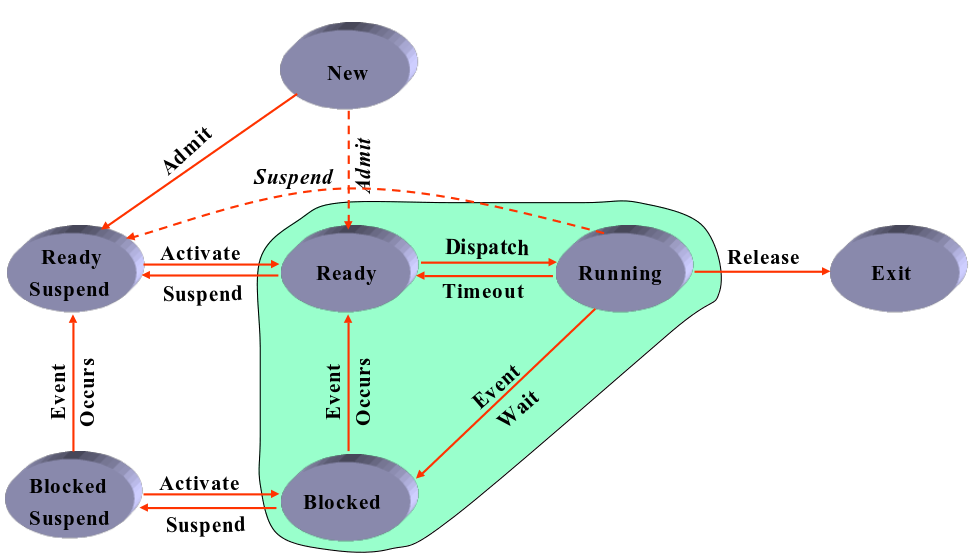
\includegraphics[width=\textwidth]{process.png}
\caption{进程状态转换的7状态模型}
\label{fig: process}
\end{figure}
\end{center}

\begin{table}[htbp]
\centering  % 表居中
\begin{tabular}{ll}  % {lccc} 表示各列元素对齐方式,left-l,right-r,center-c
\hline
运行结果 & 说明 \\
\hline
图\ref{fig: cmd} &  打印程序使用说明(所有命令格式)\\
图\ref{fig: admit0} &  执行\texttt{admit 0},收容0进程(并就绪)\\
图\ref{fig: admit1} &  执行\texttt{admit 1},收容1进程(并就绪)\\
图\ref{fig: dispatch0} &  执行\texttt{dispatch 0},调度0进程执行(从就绪队列切上CPU)\\
图\ref{fig: fork2} &  执行\texttt{fork 2},为0进程创建子进程2(子进程就绪)\\
图\ref{fig: eventwaits0} &  执行\texttt{eventwaits 0},0进程等待某事件发生,被阻塞(从CPU切下进入阻塞队列)\\
图\ref{fig: eventoccurs0} &  执行\texttt{eventoccurs 0},0进程等待的事件发生,被唤醒(由阻塞队列进入就绪队列)\\
图\ref{fig: suspend0} &  执行\texttt{suspend 0},挂起0进程\\
图\ref{fig: activate0} &  执行\texttt{activate 0},激活0进程\\
图\ref{fig: timeout0} &  执行\texttt{timeout 0},0进程超时(进入就绪队列)\\
图\ref{fig: dispatch0aftertimout0} &  执行\texttt{dispatch 0},再次调度0进程执行(从就绪队列切上CPU)\\
图\ref{fig: rebase0} &  执行\texttt{rebase 0},杀死0进程(及其所有子孙进程)\\
图\ref{fig: quit1} &  执行\texttt{quit 1},退出\\
\hline  % \hline 在此行下面画一横线
\end{tabular}
\caption{数据结构说明\label{tab: data_structure}}
\end{table}

\begin{center}
\begin{figure}[htbp]
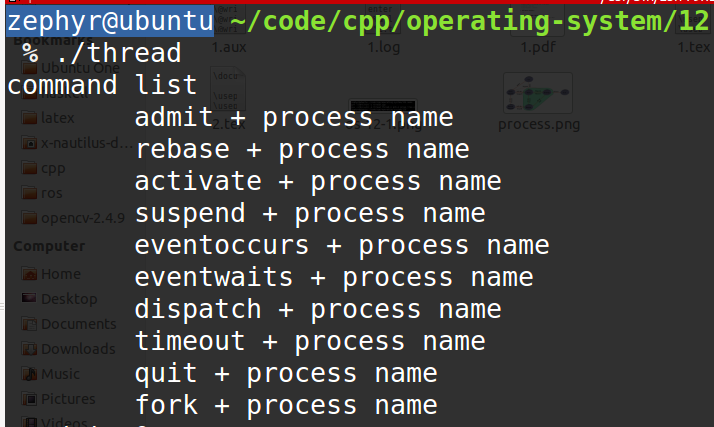
\includegraphics[width=\textwidth]{cmd.png}
\caption{\texttt{cmd}}
\label{fig: cmd}
\end{figure}
\begin{figure}[htbp]
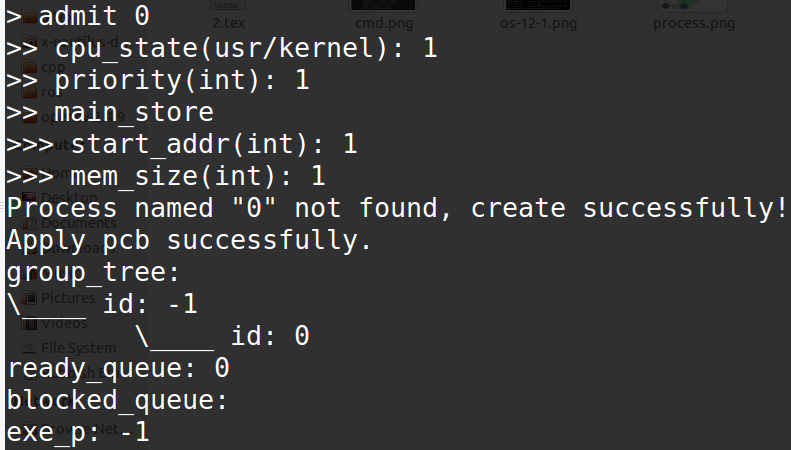
\includegraphics[width=\textwidth]{admit0.png}
\caption{\texttt{admit 0}}
\label{fig: admit0}
\end{figure}
\begin{figure}[htbp]
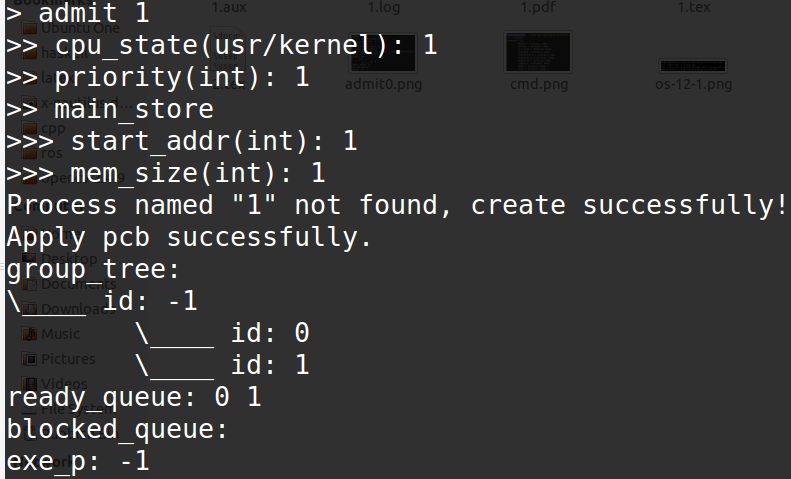
\includegraphics[width=\textwidth]{admit1.png}
\caption{\texttt{admit 1}}
\label{fig: admit1}
\end{figure}
\begin{figure}[htbp]
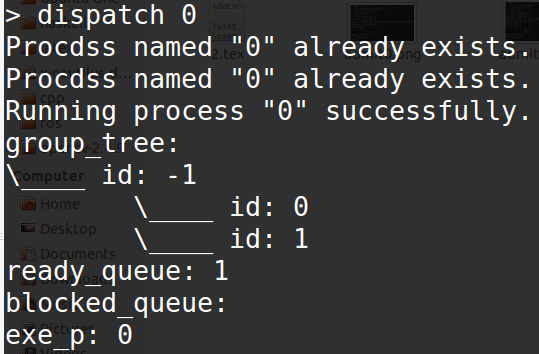
\includegraphics[width=\textwidth]{dispatch0.png}
\caption{\texttt{dispatch 0}}
\label{fig: dispatch0}
\end{figure}
\begin{figure}[htbp]
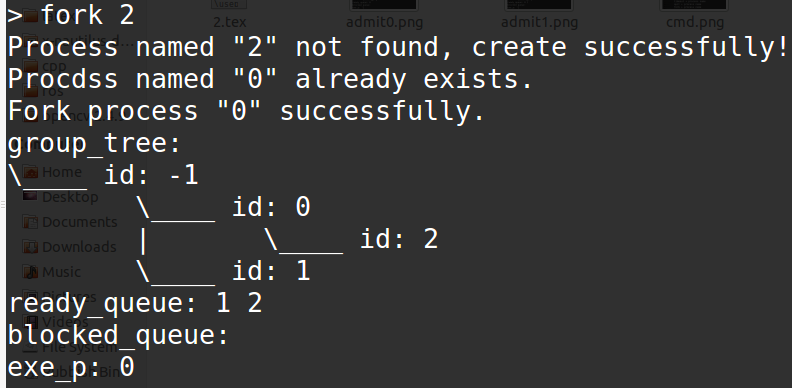
\includegraphics[width=\textwidth]{fork2.png}
\caption{\texttt{fork 2}}
\label{fig: fork2}
\end{figure}
\begin{figure}[htbp]
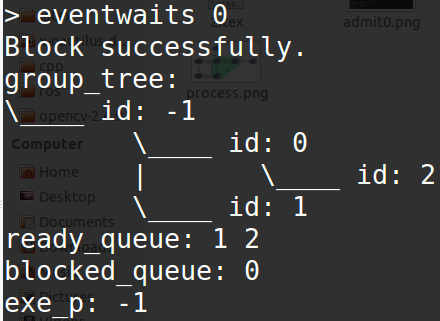
\includegraphics[width=\textwidth]{eventwaits0.png}
\caption{\texttt{eventwaits 0}}
\label{fig: eventwaits0}
\end{figure}
\begin{figure}[htbp]
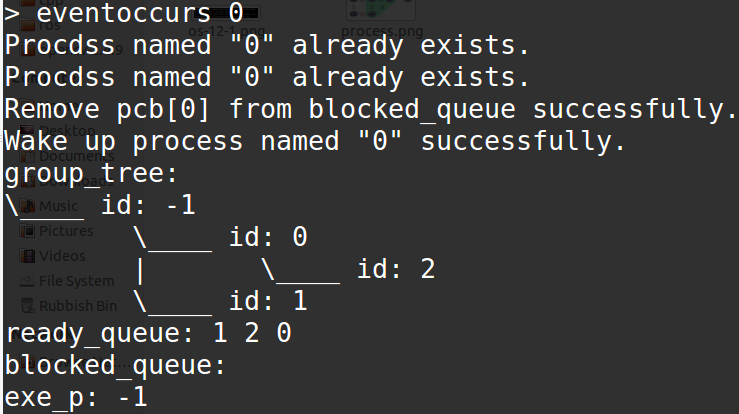
\includegraphics[width=\textwidth]{eventoccurs0.png}
\caption{\texttt{eventoccurs0}}
\label{fig: eventoccurs0}
\end{figure}
\begin{figure}[htbp]
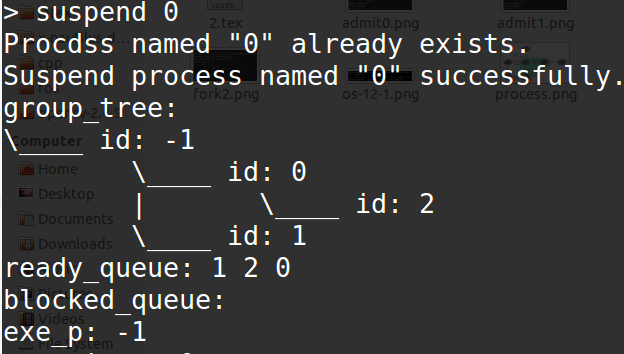
\includegraphics[width=\textwidth]{suspend0.png}
\caption{\texttt{suspend 0}}
\label{fig: suspend0}
\end{figure}
\begin{figure}[htbp]
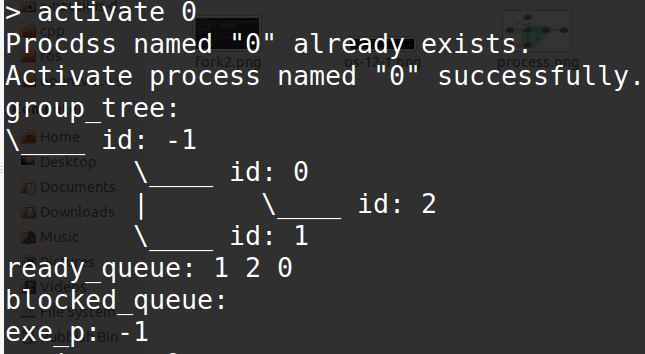
\includegraphics[width=\textwidth]{activate0.png}
\caption{\texttt{activate 0}}
\label{fig: activate0}
\end{figure}
\begin{figure}[htbp]
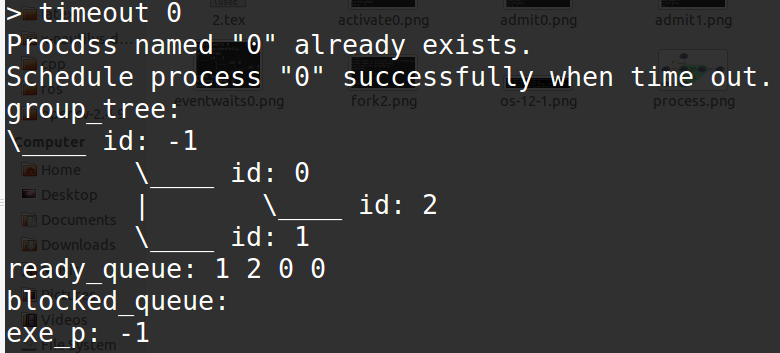
\includegraphics[width=\textwidth]{timeout0.png}
\caption{\texttt{timeout 0}}
\label{fig: timeout0}
\end{figure}
\begin{figure}[htbp]
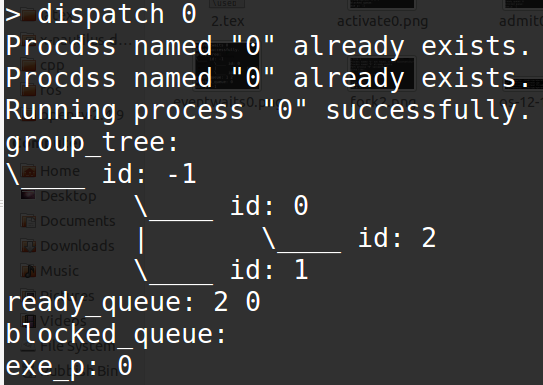
\includegraphics[width=\textwidth]{dispatch0aftertimout0.png}
\caption{\texttt{dispatch 0}}
\label{fig: dispatch0aftertimout0}
\end{figure}
\begin{figure}[htbp]
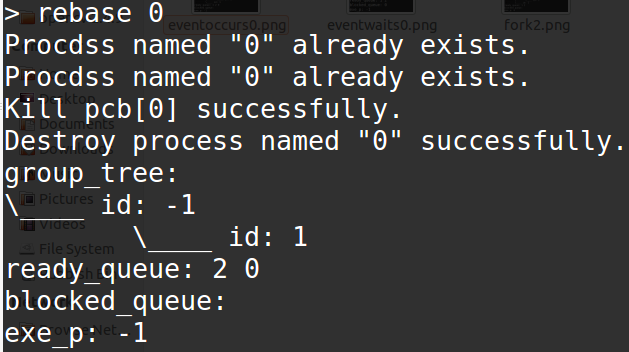
\includegraphics[width=\textwidth]{rebase0.png}
\caption{\texttt{rebase 0}}
\label{fig: rebase0}
\end{figure}
\begin{figure}[htbp]
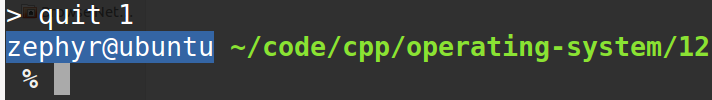
\includegraphics[width=\textwidth]{quit1.png}
\caption{\texttt{quit 1}}
\label{fig: quit1}
\end{figure}
\end{center}

\section{程序使用说明}
见表\ref{tab: use}

\begin{table}[htbp]
\centering  % 表居中
\begin{tabular}{ |l|l|l| }
\hline
\multirow{3}{*}{\texttt{admit}(收容)} & \multicolumn{2}{c|}{\texttt{cpu\_state}(CPU状态)} \\ \cline{2-3} & \multicolumn{2}{c|}{\texttt{priority}(优先级)} \\ \cline{2-3} & \multirow{2}{*}{\texttt{main\_store}(主存)} & \texttt{start\_addr}(起始地址) \\  & & \texttt{mem\_size}(占用内存大小) \\ \hline
\multicolumn{3}{|c|}{\texttt{dispatch}(调度执行)} \\ \hline
\multicolumn{3}{|c|}{\texttt{suspend}(挂起)} \\ \hline
\multicolumn{3}{|c|}{\texttt{activate}(激活)} \\ \hline
\multicolumn{3}{|c|}{\texttt{eventwaits}(等待事件发生,阻塞)} \\ \hline
\multicolumn{3}{|c|}{\texttt{eventoccurs}(等待的事件发生,唤醒)} \\ \hline
\multicolumn{3}{|c|}{\texttt{timeout}(超时,就绪)} \\ \hline
\multicolumn{3}{|c|}{\texttt{rebase}(杀死进程及其所有子孙进程)} \\ \hline
\multicolumn{3}{|c|}{\texttt{fork}(创建子进程)} \\ \hline
\multicolumn{3}{|c|}{\texttt{quit}(退出)} \\ \hline
\end{tabular}
\caption{程序使用说明\label{tab: use}}
\end{table}

\end{document}
